% Options for packages loaded elsewhere
\PassOptionsToPackage{unicode}{hyperref}
\PassOptionsToPackage{hyphens}{url}
%
\documentclass[
]{article}
\usepackage{amsmath,amssymb}
\usepackage{iftex}
\ifPDFTeX
  \usepackage[T1]{fontenc}
  \usepackage[utf8]{inputenc}
  \usepackage{textcomp} % provide euro and other symbols
\else % if luatex or xetex
  \usepackage{unicode-math} % this also loads fontspec
  \defaultfontfeatures{Scale=MatchLowercase}
  \defaultfontfeatures[\rmfamily]{Ligatures=TeX,Scale=1}
\fi
\usepackage{lmodern}
\ifPDFTeX\else
  % xetex/luatex font selection
\fi
% Use upquote if available, for straight quotes in verbatim environments
\IfFileExists{upquote.sty}{\usepackage{upquote}}{}
\IfFileExists{microtype.sty}{% use microtype if available
  \usepackage[]{microtype}
  \UseMicrotypeSet[protrusion]{basicmath} % disable protrusion for tt fonts
}{}
\makeatletter
\@ifundefined{KOMAClassName}{% if non-KOMA class
  \IfFileExists{parskip.sty}{%
    \usepackage{parskip}
  }{% else
    \setlength{\parindent}{0pt}
    \setlength{\parskip}{6pt plus 2pt minus 1pt}}
}{% if KOMA class
  \KOMAoptions{parskip=half}}
\makeatother
\usepackage{xcolor}
\usepackage[margin=1in]{geometry}
\usepackage{color}
\usepackage{fancyvrb}
\newcommand{\VerbBar}{|}
\newcommand{\VERB}{\Verb[commandchars=\\\{\}]}
\DefineVerbatimEnvironment{Highlighting}{Verbatim}{commandchars=\\\{\}}
% Add ',fontsize=\small' for more characters per line
\usepackage{framed}
\definecolor{shadecolor}{RGB}{248,248,248}
\newenvironment{Shaded}{\begin{snugshade}}{\end{snugshade}}
\newcommand{\AlertTok}[1]{\textcolor[rgb]{0.94,0.16,0.16}{#1}}
\newcommand{\AnnotationTok}[1]{\textcolor[rgb]{0.56,0.35,0.01}{\textbf{\textit{#1}}}}
\newcommand{\AttributeTok}[1]{\textcolor[rgb]{0.13,0.29,0.53}{#1}}
\newcommand{\BaseNTok}[1]{\textcolor[rgb]{0.00,0.00,0.81}{#1}}
\newcommand{\BuiltInTok}[1]{#1}
\newcommand{\CharTok}[1]{\textcolor[rgb]{0.31,0.60,0.02}{#1}}
\newcommand{\CommentTok}[1]{\textcolor[rgb]{0.56,0.35,0.01}{\textit{#1}}}
\newcommand{\CommentVarTok}[1]{\textcolor[rgb]{0.56,0.35,0.01}{\textbf{\textit{#1}}}}
\newcommand{\ConstantTok}[1]{\textcolor[rgb]{0.56,0.35,0.01}{#1}}
\newcommand{\ControlFlowTok}[1]{\textcolor[rgb]{0.13,0.29,0.53}{\textbf{#1}}}
\newcommand{\DataTypeTok}[1]{\textcolor[rgb]{0.13,0.29,0.53}{#1}}
\newcommand{\DecValTok}[1]{\textcolor[rgb]{0.00,0.00,0.81}{#1}}
\newcommand{\DocumentationTok}[1]{\textcolor[rgb]{0.56,0.35,0.01}{\textbf{\textit{#1}}}}
\newcommand{\ErrorTok}[1]{\textcolor[rgb]{0.64,0.00,0.00}{\textbf{#1}}}
\newcommand{\ExtensionTok}[1]{#1}
\newcommand{\FloatTok}[1]{\textcolor[rgb]{0.00,0.00,0.81}{#1}}
\newcommand{\FunctionTok}[1]{\textcolor[rgb]{0.13,0.29,0.53}{\textbf{#1}}}
\newcommand{\ImportTok}[1]{#1}
\newcommand{\InformationTok}[1]{\textcolor[rgb]{0.56,0.35,0.01}{\textbf{\textit{#1}}}}
\newcommand{\KeywordTok}[1]{\textcolor[rgb]{0.13,0.29,0.53}{\textbf{#1}}}
\newcommand{\NormalTok}[1]{#1}
\newcommand{\OperatorTok}[1]{\textcolor[rgb]{0.81,0.36,0.00}{\textbf{#1}}}
\newcommand{\OtherTok}[1]{\textcolor[rgb]{0.56,0.35,0.01}{#1}}
\newcommand{\PreprocessorTok}[1]{\textcolor[rgb]{0.56,0.35,0.01}{\textit{#1}}}
\newcommand{\RegionMarkerTok}[1]{#1}
\newcommand{\SpecialCharTok}[1]{\textcolor[rgb]{0.81,0.36,0.00}{\textbf{#1}}}
\newcommand{\SpecialStringTok}[1]{\textcolor[rgb]{0.31,0.60,0.02}{#1}}
\newcommand{\StringTok}[1]{\textcolor[rgb]{0.31,0.60,0.02}{#1}}
\newcommand{\VariableTok}[1]{\textcolor[rgb]{0.00,0.00,0.00}{#1}}
\newcommand{\VerbatimStringTok}[1]{\textcolor[rgb]{0.31,0.60,0.02}{#1}}
\newcommand{\WarningTok}[1]{\textcolor[rgb]{0.56,0.35,0.01}{\textbf{\textit{#1}}}}
\usepackage{longtable,booktabs,array}
\usepackage{calc} % for calculating minipage widths
% Correct order of tables after \paragraph or \subparagraph
\usepackage{etoolbox}
\makeatletter
\patchcmd\longtable{\par}{\if@noskipsec\mbox{}\fi\par}{}{}
\makeatother
% Allow footnotes in longtable head/foot
\IfFileExists{footnotehyper.sty}{\usepackage{footnotehyper}}{\usepackage{footnote}}
\makesavenoteenv{longtable}
\usepackage{graphicx}
\makeatletter
\def\maxwidth{\ifdim\Gin@nat@width>\linewidth\linewidth\else\Gin@nat@width\fi}
\def\maxheight{\ifdim\Gin@nat@height>\textheight\textheight\else\Gin@nat@height\fi}
\makeatother
% Scale images if necessary, so that they will not overflow the page
% margins by default, and it is still possible to overwrite the defaults
% using explicit options in \includegraphics[width, height, ...]{}
\setkeys{Gin}{width=\maxwidth,height=\maxheight,keepaspectratio}
% Set default figure placement to htbp
\makeatletter
\def\fps@figure{htbp}
\makeatother
\setlength{\emergencystretch}{3em} % prevent overfull lines
\providecommand{\tightlist}{%
  \setlength{\itemsep}{0pt}\setlength{\parskip}{0pt}}
\setcounter{secnumdepth}{-\maxdimen} % remove section numbering
\usepackage{booktabs}
\usepackage{longtable}
\usepackage{array}
\usepackage{multirow}
\usepackage{wrapfig}
\usepackage{float}
\usepackage{colortbl}
\usepackage{pdflscape}
\usepackage{tabu}
\usepackage{threeparttable}
\usepackage{threeparttablex}
\usepackage[normalem]{ulem}
\usepackage{makecell}
\usepackage{xcolor}
\ifLuaTeX
  \usepackage{selnolig}  % disable illegal ligatures
\fi
\usepackage{bookmark}
\IfFileExists{xurl.sty}{\usepackage{xurl}}{} % add URL line breaks if available
\urlstyle{same}
\hypersetup{
  hidelinks,
  pdfcreator={LaTeX via pandoc}}

\author{}
\date{\vspace{-2.5em}}

\begin{document}

\section{EXPERIMENTOS FATORIAIS}\label{experimentos-fatoriais}

\subsection{Introdução}\label{introduuxe7uxe3o}

Os experimentos simples, realizados de acordo com o delineamento
inteiramente casualizado (DIC) ou em blocos casualizados (DBC), são
utilizados para testar os efeitos de apenas um tipo de
\textbf{tratamento}, ou \textbf{fator}, sendo os demais mantidos
constantes.

Assim, por exemplo, num experimento de comparação de inseticidas em
relação ao controle de uma determinada praga, devemos manter constante a
dosagem, o método de aplicação, os tratos culturais, etc.

Porém, há casos em que necessitamos testar simultaneamente os efeitos de
dois ou mais tipos de tratamentos (fatores) para obtermos resultados de
interesse prático. Por exemplo, supondo que desejamos testar \(3\)
inseticidas, \(2\) métodos de aplicação e \(4\) dosagens, teremos então
um \textbf{experimento fatorial} de \(3\times2\times4\).

Os experimentos fatoriais são aqueles que nos permitem estudar,
simultaneamente, os efeitos de dois ou mais tipos de fatores. Assim,
eles devem ser instalados em um dos delineamentos já estudados (DIC,
DBC, etc.).

Estes experimentos são utilizados em quase todos os campos de
investigação e são bastante úteis em pesquisas iniciais, nas quais pouco
se conhece a respeito de uma série de fatores.

\textbf{O número de tratamentos nos experimentos fatoriais consiste de
todas as combinações possíveis dos níveis dos fatores}.

Por exemplo, se estamos interessados em testar o efeito de \(3\)
inseticidas, cada um dos quais em \(4\) doses, teremos os \(12\)
tratamentos seguintes.

\[
\begin{array}{} 
I_1 D_1  & I_2D_1  & I_3D_1 \\
I_1D_2  & I_2D_2  & I_3D_2 \\
I_1D_3  & I_2D_3  & I_3D_3 \\ 
I_1D_4  & I_2D_4  & I_3D_4 \end{array}
\]

Neste caso, representamos o esquema fatorial como:
\(\text{Fatorial }3 \times 4\) com \(3\) inseticidas e \(4\) dosagens.

\textbf{As subdivisões de um fator são denominados NÍVEIS desse fator}.

Então, no exemplo anterior, o fator \textbf{Inseticida} ocorrem em
\textbf{3 níveis}, e o fator \textbf{Dosagem} ocorre em \textbf{4
níveis}.

Assim, no ensaio acima, podemos obter conclusões sobre qual o melhor
inseticida, qual a melhor dosagem e qual a melhor dosagem para cada
inseticida.

Vamos então apresentar algumas definições necessárias ao bom
entendimento dos ensaios fatoriais.

Supondo que temos \(2\) fatores \textbf{A} e \textbf{B} cada um dos
quais em dois níveis \((0 \text{ e } 1)\), presença e ausência,
respectivamente, e que os resultados obtidos foram os seguintes:

\begin{longtable}[]{@{}cccc@{}}
\toprule\noalign{}
& \(B_0\) & \(B_1\) & Total \\
\midrule\noalign{}
\endhead
\bottomrule\noalign{}
\endlastfoot
\(A_0\) & \(3\) & \(7\) & \(10\) \\
\(A_1\) & \(9\) & \(18\) & \(27\) \\
\textbf{Total} & \(12\) & \(25\) & \(37\) \\
\end{longtable}

\href{https://github.com/arpanosso/experimentacao-agricola-unesp-fcav/raw/master/data/interação.xlsx}{DOWNLOAD}

\subsection{Efeito simples de um
fator}\label{efeito-simples-de-um-fator}

É uma medida da variação que ocorre com a variável resposta
(característica em estudo) correspondente a variação nos níveis desse
fator, em cada um dos níveis do outro fator.

Efeito de \(A\) dentro de \(B_0 = A_1B_0-A_0B_0 = 9 -3 = 6\)

Efeito de \(A\) dentro de \(B_1 = A_1B_1-A_0B_1 = 18-7 = 11\)

Efeito de \(B\) dentro de \(A_0 = A_0B_1-A_0B_0=7-3=4\)

Efeito de \(B\) dentro de \(A_1 = A_1B_1-A_1B_0 = 18-9=9\)

\subsection{Efeito principal de um
fator}\label{efeito-principal-de-um-fator}

É uma medida da variação que ocorre com a variável resposta
correspondente às variações nos níveis em média de todos os níveis do
outro fator.

\textbf{Efeito Principal de A}

\[
A = \frac{\text{Ef. de A d. }B_0+\text{Ef. de A d. }B_1}{2}=\frac{6+11}{2}=8,5
\] ou ainda:

\(A = \frac{A_1B_0+A_1B_1}{2}-\frac{A_0B_0+A_0B_1}{2} = \frac{9+18}{2}-\frac{3+7}{2} = 13,5-5,0=8,5\)

\textbf{Efeito Principal de B}

\[
B = \frac{\text{Ef. de B d. }A_0+\text{Ef. de B d. }A_1}{2}=\frac{4+9}{2}=6,5
\]

ou ainda:

\(B = \frac{A_0B_1+A_1B_1 }{2}-\frac{A_0B_0+A _1B_0}{2}  = \frac{7+18}{2}-\frac{3+9}{2} = 12,5-6,0=6,5\)

\textbf{Portanto, o efeito principal de um fator é a média dos efeitos
simples desse fator}

\subsection{Efeito da interação entre
fatores}\label{efeito-da-interauxe7uxe3o-entre-fatores}

É uma medida da variação que ocorre com o efeito simples de um fator ao
passar de um nível a outro do outro fator.

\textbf{Efeito da Interação} \(A \times B\)

\[
A \times B = \frac{A\;d.\;B_1-A\;d.\;B_0}{2} = \frac{(A_1B_1-A_0B_1)-(A_1B_0-A_0B_0)}{2}=\frac{11-6}{2}=2,5
\]

\textbf{Efeito da Interação} \(B \times A\)

\(B \times A = \frac{B\;d.\;A_1-B\;d.\;A_0}{2} = \frac{(A_1B_1-A_1B_0)-(A_0B_1-A_0B_0)}{2}=\frac{9-4}{2} =  2,5\)

Note que o efeito da Interação \(A \times B = B \times A\).

\subsection{Vantagens dos experimentos
fatoriais}\label{vantagens-dos-experimentos-fatoriais}

\begin{itemize}
\item
  Permite estudar os efeito simples, o efeito principal e o efeito da
  interação entre fatores.
\item
  Todas as parcelas experimentais entram no cálculo dos efeitos
  principais e interações, razão pela qual as médias dos níveis dos
  fatores são calculadas com um maior número de repetições.
\end{itemize}

\subsection{Desvantagens dos experimentos
fatoriais}\label{desvantagens-dos-experimentos-fatoriais}

\begin{itemize}
\item
  A análise estatística é trabalhosa, e a interpretação dos resultados
  torna-se mais difícil à medida que aumentam o número de fatores e de
  níveis.
\item
  Como os tratamentos devem conter todas as combinações possíveis dos
  fatores em seus diversos níveis, o número de tratamentos aumenta
  rapidamente, e às vezes devido à exigência de homogeneidade dentro dos
  blocos, não podemos utilizar o delinemamento em blocos completos
  casualizados.
\item
  Sendo os tratamentos constituídos de todas as combinações possíveis
  dos fatores em seus diversos níveis, para que haja um balanceamento
  estatístico, às vezes algumas das combinações não tem interesse
  prático, mas devem ser mantidas para não quebrar o balanceamento.
\end{itemize}

\subsection{Classificação dos experimentos
fatoriais}\label{classificauxe7uxe3o-dos-experimentos-fatoriais}

\textbf{Fatoriais de série \(2^N\)}

Nesta série são enquadrados os experimentos fatoriais em que são
estudados os efeitos de \(N\) fatores cada um em \(2\) níveis.

BASE = Nº de Níveis\\
EXPOENTE = Nº de Fatores

Exemplos: \[
2^2 \Rightarrow \text{2 Fatores em 2 Níveis} \\
2^3 \Rightarrow \text{3 Fatores em 2 Níveis} \\
2^4 \Rightarrow \text{4 Fatores em 2 Níveis} \\
\]

etc.

\textbf{Fatoriais de série \(3^N\)}

Nesta série são enquadrados os experimentos fatoriais em que são
estudados os efeitos de \(N\) fatores cada um em \(3\) níveis.

Exemplos: \[
3^2 \Rightarrow \text{2 Fatores em 3 Níveis} \\
3^3 \Rightarrow \text{3 Fatores em 3 Níveis} \\
3^4 \Rightarrow \text{4 Fatores em 3 Níveis} \\
\] etc.

\textbf{Fatoriais de série mista}

Nesta série são enquadrado os fatoriais em que os fatores ocorrem em
número diferente de níveis:

Exemplo: \[
4\times 3\times 2 \Rightarrow \begin{cases} \text{1º Fator em 4 Níveis }\\ \text{2º Fator em 3 Níveis } \\ \text{3º Fator em 2 Níveis } \end{cases}
\]

\subsection{Casualização dos
tratamentos}\label{casualizauxe7uxe3o-dos-tratamentos}

Para exemplificar a casualização dos tratamentos, vamos supor um
experimento fatorial \(3 \times 2\), com \(3\) variedades de milho
(\(V_1,V_2,V_3\)) e \(2\) níveis de adubação com \(P_2O_5\)
(\(P_1 e\; P_2\)). Se o experimento fosse instalado de acordo com o
delineamento em blocos casualizados, com \(4\) repetições, teríamos:

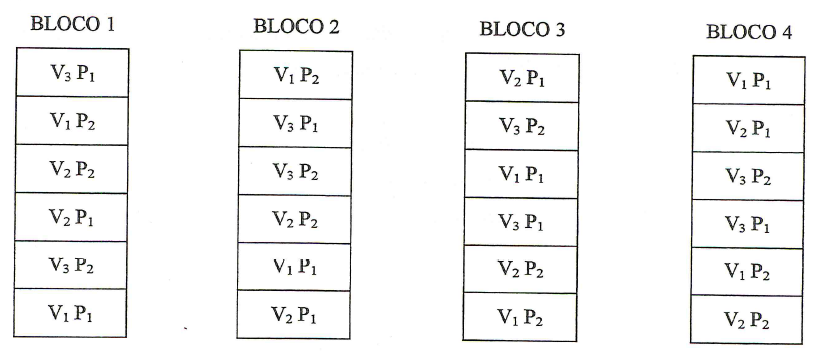
\includegraphics{Casuali.png}

O esquema da análise de variância preliminar deste ensaio será o
seguinte:

\begin{longtable}[t]{lr}
\toprule
Causas de Variação & GL\\
\midrule
Tratamentos & 5\\
Blocos & 3\\
Resíduos & 15\\
\textbf{Total} & \textbf{23}\\
\bottomrule
\end{longtable}

Após a análise de variância preliminar, os graus de liberdade de
tratamentos devem ser desdobrados de acordo com o esquema fatorial
\(3 \times 2\), da seguinte maneira:

\begin{longtable}[t]{ll}
\toprule
Causas de Variação & GL\\
\midrule
Variedades (V) & 2\\
Adubação (P) & 1\\
Interação (VxP) & 2\\
\textbf{(Tratamentos)} & \textbf{5}\\
Blocos & 3\\
\addlinespace
Resíduos & 15\\
\textbf{Total} & \textbf{23}\\
\bottomrule
\end{longtable}

\subsection{\texorpdfstring{Análise de variância de um experimento
fatorial com \(2\) fatores com interação não
significativa}{Análise de variância de um experimento fatorial com 2 fatores com interação não significativa}}\label{anuxe1lise-de-variuxe2ncia-de-um-experimento-fatorial-com-2-fatores-com-interauxe7uxe3o-nuxe3o-significativa}

Para a obtenção da análise de variância, vamos utlizar os dados
adaptados do trabalho ``Ensaios em condições de casa-de-vegetação para
controle químico do `damping-off' em \emph{Eucalyptus saligna} Sm.'',
realizado por KRUGNER; CARVALHO (1971) e publicado em IPEF, n 2/3
p.~97-113. O ensaio foi realizado no delineamento inteiramente
casualizado, com \(3\) repetições e foram estudados os efeitos sobre a
altura média das mudas de \emph{Eucalytus saligna}, dos fatores:

\textbf{Tratamento do solo (S)}, sendo:\\
\(S_1=\text{Vapam}\)\\
\(S_2=\text{Brometo de metila}\)\\
\(S_3=\text{PCNB}\)\\
\(S_4=\text{Testemunha}\)

\textbf{Pulverização} com fungicida em pós emergência, sendo:\\
\(F_0 = \text{Sem fungicida}\)\\
\(F_1 = \text{Com fungicida}\)

Os dados podem ser encontrados online em
\href{https://raw.githubusercontent.com/arpanosso/ExpAgr_2020/master/dados/solofungi.txt}{solofungi.txt}

As alturas médias de mudas (\emph{cm}) \(28\) dias após a semeadura
foram:

\begin{longtable}[]{@{}lcccr@{}}
\toprule\noalign{}
Tratamentos & Rep.1 & Rep.2 & Rep.3 & Total \\
\midrule\noalign{}
\endhead
\bottomrule\noalign{}
\endlastfoot
\(S_1F_0\) & 4,65 & 5,18 & 5,52 & 15,35 \\
\(S_1F_1\) & 4,86 & 4,81 & 4,51 & 14,18 \\
\(S_2F_0\) & 4,55 & 5,16 & 6,00 & 15,71 \\
\(S_2F_1\) & 4,73 & 5,51 & 5,09 & 15,33 \\
\(S_3F_0\) & 2,68 & 2,65 & 2,56 & 7,89 \\
\(S_3F_1\) & 2,90 & 2,71 & 2,93 & 8,54 \\
\(S_4F_0\) & 3,48 & 2,75 & 3,06 & 9,29 \\
\(S_4F_1\) & 2,65 & 2,47 & 2,83 & 7,95 \\
\textbf{Total} & & & & \textbf{94,24} \\
\end{longtable}

\textbf{Dados
originais}:\href{https://github.com/arpanosso/experimentacao-agricola-unesp-fcav/raw/master/data/dados_altura_mudas.xlsx}{DOWNLOAD}

\subsection{Obtenção da análise de
variância}\label{obtenuxe7uxe3o-da-anuxe1lise-de-variuxe2ncia}

O ensaio foi montado de acordo com o delineamento inteiramente
casualizado, e, portanto, a análise de variância preliminar, obtida de
maneira usual, foi a seguinte:

\[
\begin{aligned}
SQ_{Total} &= (4,65^2+5,18^2+ \dots +2,83^2) - \frac{94,24^2}{8 \cdot 3} \\
           & = 403,2566 - 370,0491 \\
           &= 33,2075 \\
\\
\\
SQ_{Trat} &= \frac{1}{3}(15,35^2+14,18^2+ \dots +7,95^2) - \frac{94,24^2}{8 \cdot 3} \\
           & = 401,0061 - 370,0491 \\
           &= 31,0170 \\
\\
\\
SQ_{Res} &= SQ_{Total} - SQ_{Trat} \\
           & = 33,2075 - 31,0170 \\
           &= 2,1905
\end{aligned}
\]

Quadro da análise de variância preliminar:

\begin{longtable}[t]{lrlll}
\toprule
Causas de Variação & GL & SQ & QM & F\\
\midrule
Tratamentos & 7 & 31,0170 & 4,4310 & 32,37**\\
Resíduos & 16 & 2,1905 & 0,1369 & \\
\textbf{Total} & \textbf{23} & \textbf{33,20175} & \textbf{} & \textbf{}\\
\bottomrule
\end{longtable}

\textbf{Conclusão}: O teste \(F\) foi significativo ao nível de \(1\%\)
de probabilidade, logo, rejeitamos a hipótese da nulidade (\(H_0\)), e
concluímos que os tratamentos possuem efeitos diferentes sobre a altura
das mudas de \emph{Eucalyptus saligna}, com um grau de confiança
superior a \(99\%\) de probabilidade.

Devemos agora desdobrar a soma de quadrados e os graus de liberdade de
tratamentos para estudar os efeitos principais e a interação entre os
fatores.

Para facilitar os cálculos, utilizamos um quadro auxiliar como o
seguinte:

\begin{longtable}[]{@{}lccccc@{}}
\toprule\noalign{}
\((3)\) & \(S_1\) & \(S_1\) & \(S_1\) & \(S_1\) & \textbf{Total} \\
\midrule\noalign{}
\endhead
\bottomrule\noalign{}
\endlastfoot
\(F_0\) & 15,35 & 15,71 & 7,89 & 9,29 & \textbf{48,24} \\
\(F_1\) & 14,18 & 15,33 & 8,54 & 7,95 & \textbf{46,00} \\
\textbf{Total} & \textbf{29,53} & \textbf{31,04} & \textbf{16,43} &
\textbf{17,24} & \textbf{94,24} \\
\end{longtable}

Então, as somas de quadrados são obtidas da seguinte maneira:

\textbf{1. Soma de quadrados devido ao efeito de Tratamento do Solo:} \[
\begin{aligned}
SQ_{Ef.Trat.Solo} &= \frac{1}{r_s}(T_{S_1}^2+T_{S_2}^2+T_{S_3}^2+T_{S_4}^2) - C \\
                  &= \frac{1}{6}(29,53^2+31,04^2+16,43^2+17,24^2) - \frac{94,24^2}{24} \\
                  &= 30,3951
\end{aligned}
\]

\textbf{2. Soma de quadrados devido ao efeito de Fungicidas:}

\[
\begin{aligned}
SQ_{Ef.Fung.} &= \frac{1}{r_F}(T_{F_0}^2+T_{F_1}^2) - C \\
                  &= \frac{1}{12}(48,24^2+46,00^2) - \frac{94,24^2}{24} \\
                  &= 0,2091
\end{aligned}
\]

\textbf{3. Soma de quadrados devido ao efeito da Interação Tratamento do
Solo x Fungicida:}

\[
\begin{aligned}
SQ_{Interação\;S\times F} &= SQ_{S,F}-SQ_{Ef.Trat.Solo}-SQ_{Ef.Fungicida} \\ \\
& \text{assim, calculamos } SQ_{S,F}: \\ 
SQ_{S,F} &= \frac{1}{r_{SF}}(T_{S_1F_0}^2+T_{S_1F_1}^2+\cdots +T_{S_4F_1}^2) - C \\
                  &= \frac{1}{3}(15,35^2+14,18^2+\cdots + 7,95^2) - \frac{94,24^2}{24} \\
                  &= 31,0170
\end{aligned}
\]

Portanto,

\[
\begin{aligned}
SQ_{Interação\;S\times F} &= SQ_{S,F}-SQ_{S}-SQ_{F} \\
SQ_{Interação\;S\times F} &= 31,0170-30,3951-0,2091 \\
&= 0,4128
\end{aligned}
\]

Portanto, temos o seguinte quadro de análise de variância:

\begin{longtable}[t]{lllll}
\toprule
Causas de Variação & GL & SQ & QM & F\\
\midrule
Tratamento de solo (S) & 3 & 30,3951 & 10,1317 & 74,00**\\
Fungicida (F) & 1 & 0,2091 & 0,2091 & 1,53ns\\
Interação (SxF) & 3 & 0,4128 & 0,1376 & 1,01ns\\
\textbf{(Tratamentos)} & \textbf{7} & \textbf{31,0170} & \textbf{} & \textbf{}\\
Resíduos & 16 & 2,1905 & 0,1369 & \\
\addlinespace
\textbf{Total} & \textbf{23} & \textbf{33,2075} & \textbf{} & \textbf{}\\
\bottomrule
\end{longtable}

Valores de \(F\) da tabela para Trat. do solo (\(3 \times 16 GL\)):
\(\begin{cases}5\%=3,24 \\ 1\%=5,29 \end{cases}\)

Valores de \(F\) da tabela para Fungicida (\(1 \times 16 GL\)):
\(\begin{cases}5\%=4,49 \\ 1\%=8,53 \end{cases}\)

Valores de \(F\) da tabela para Interação \(S\times F\)
(\(3 \times 16 GL\)): \(\begin{cases}5\%=3,24 \\ 1\%=5,29 \end{cases}\)

\textbf{Conclusões}

\textbf{Para efeito de Tratamento do solo}: O teste foi significativo ao
nível de \(1\%\) de probabilidade, indicando que devemos rejeitar
\(H_0\) e concluir que os tratamentos do solo possuem efeitos diferentes
sobre a altura de mudas de eucalipto.

\textbf{Para efeito de Fungicida}: O teste não foi significativo ao
nível de \(5\%\) de probabilidade, indicando que não devemos rejeitar
\(H_0\) e concluir que a aplicação ou não de fungicida em pós-emergência
não possui efeito sobre a altura de mudas de eucalipto.

\textbf{Para efeito da Interação (S \(\times\) F)}: O teste não foi
significativo ao nível de \(5\%\) de probabilidade, indicando que não
devemos rejeitar \(H_0\) e concluir que os tratamentos de solo agem de
maneira independente do fungicida sobre a altura das mudas de eucalipto.

Portanto, como a Interação S\(\times\)F foi não significativa, podemos
estudar os efeitos principais dos fatores independentemente um do outro.

Para complementar a análise de variância, e obter conclusões mais
específicas sobre o efeito de cada um dos fatores, podemos utilizar os
testes de comparação de médias.

\subsection{Cálculo das médias de Tratamento do Solo e erros padrões das
médias}\label{cuxe1lculo-das-muxe9dias-de-tratamento-do-solo-e-erros-padruxf5es-das-muxe9dias}

\[
\hat{m_{S_1}} = \frac{T_{S_1}}{r_{S_1}}=\frac{29,53}{6}=4,92\;cm \\
\hat{m_{S_2}} = \frac{T_{S_2}}{r_{S_2}}=\frac{31,04}{6}=5,17\;cm \\
\hat{m_{S_3}} = \frac{T_{S_3}}{r_{S_3}}=\frac{16,43}{6}=2,74\;cm \\
\hat{m_{S_4}} = \frac{T_{S_4}}{r_{S_4}}=\frac{17,24}{6}=2,87\;cm
\]

O erro padrão destas médias será:

\[
s(\hat{m})=\sqrt{\frac{QM_{Res}}{r_S}}=\sqrt{\frac{0,1369}{6}} = 0,15\;cm
\]

\textbf{Teste de Tukey para comparar as médias de tratamento do solo}

\[
DMS=q_{(4\times16)}\cdot s(\hat{m})=4,05 \cdot 0,15 = 0,61\; cm
\]

\begin{longtable}[]{@{}lccc@{}}
\toprule\noalign{}
- & \(\hat{m_{S_1}}\) & \(\hat{m_{S_4}}\) & \(\hat{m_{S_3}}\) \\
\midrule\noalign{}
\endhead
\bottomrule\noalign{}
\endlastfoot
\(\hat{m_{S_2}}\) & \(0,25\) & \(2,30^*\) & \(2,43^*\) \\
\(\hat{m_{S_1}}\) & - & \(2,05^*\) & \(2,18^*\) \\
\(\hat{m_{S_4}}\) & - & - & \(0,13\) \\
\end{longtable}

ou ainda:

\[
\hat{m_{S_2}} = 5,17\;cm -a\\
\hat{m_{S_1}} = 4,92\;cm -a\\
\hat{m_{S_4}} = 2,87\;cm -b\\
\hat{m_{S_3}} = 2,74\;cm -b\\
\]

\textbf{Conclusão}: Médias seguidas pela mesma letra não diferem entre
sim pelo teste de Tukey ao nível de \(5\%\) de probabilidade.

\subsection{Cálculo das médias de Fungicidas e erros padrões das
médias}\label{cuxe1lculo-das-muxe9dias-de-fungicidas-e-erros-padruxf5es-das-muxe9dias}

\[
\hat{m_{F_0}} = \frac{T_{F_0}}{r_{F_0}}=\frac{48,24}{12}=4,02\;cm \\
\hat{m_{F_1}} = \frac{T_{F_1}}{r_{F_1}}=\frac{46,00}{12}=3,83\;cm 
\]

O erro padrão destas médias será:

\[
s(\hat{m})=\sqrt{\frac{QM_{Res}}{r_F}}=\sqrt{\frac{0,1369}{12}} = 0,11\;cm
\]

\textbf{Teste de Tukey para comparar as médias de Fungicidas}

Note que não houve diferença significativa entre os tratamentos com e
sem fungicidas e, portanto, não há necessidade de se comparar essas
médias. Porém, caso quiséssemos compara-lás pelo teste de Tukey,
teríamos:

\[
DMS=q_{(2\times1 6)}\cdot s(\hat{m})=3.00 \cdot 0,11 = 0,32\; cm \\
\hat{Y}=\hat{m}_{F_0}-\hat{m}_{F_1}=4,02-3,83=0,19 \; cm
\]

Portanto, como \(\hat{Y}< DMS \Rightarrow \hat{m}_{F_0}\) não difere de
\(\hat{m}_{F_1}\)

\subsection{Cálculo do coeficiente de variação do
experimento}\label{cuxe1lculo-do-coeficiente-de-variauxe7uxe3o-do-experimento}

\[
CV=100\cdot \frac{\sqrt{QM_{res}}}{\hat{m}}=100\cdot \frac{0,3700}{3,9267}=9,42\%
\]

\textbf{Aplicação no R}


\includegraphics{R.png}

\textbf{Utilizando as funções básicas e o pacote agricolae}

\begin{Shaded}
\begin{Highlighting}[]
\CommentTok{\# Carregando o pacote para análise de variância}
\FunctionTok{library}\NormalTok{(agricolae)}
\FunctionTok{library}\NormalTok{(tidyverse)}
\end{Highlighting}
\end{Shaded}

\begin{verbatim}
## -- Attaching core tidyverse packages ------------------------ tidyverse 2.0.0 --
## v dplyr     1.1.4     v readr     2.1.5
## v forcats   1.0.0     v stringr   1.5.1
## v ggplot2   3.5.1     v tibble    3.2.1
## v lubridate 1.9.3     v tidyr     1.3.1
## v purrr     1.0.2     
## -- Conflicts ------------------------------------------ tidyverse_conflicts() --
## x dplyr::filter()     masks stats::filter()
## x dplyr::group_rows() masks kableExtra::group_rows()
## x dplyr::lag()        masks stats::lag()
## i Use the conflicted package (<http://conflicted.r-lib.org/>) to force all conflicts to become errors
\end{verbatim}

\begin{Shaded}
\begin{Highlighting}[]
\CommentTok{\# Definindo o caminho do banco de dados}
\NormalTok{caminho}\OtherTok{\textless{}{-}}\StringTok{"https://raw.githubusercontent.com/arpanosso/ExpAgr\_2020/master/dados/solofungi.txt"}

\CommentTok{\# Entrada da dados}
\NormalTok{dados}\OtherTok{\textless{}{-}}\FunctionTok{read.table}\NormalTok{(caminho,}\AttributeTok{h=}\ConstantTok{TRUE}\NormalTok{)}

\CommentTok{\#Guardando os fatores (tratamentos de solo e fungicidas) e a variável resposta (y)}
\NormalTok{solos}\OtherTok{\textless{}{-}}\FunctionTok{as.factor}\NormalTok{(dados}\SpecialCharTok{$}\NormalTok{S)}
\NormalTok{fungicida}\OtherTok{\textless{}{-}}\FunctionTok{as.factor}\NormalTok{(dados}\SpecialCharTok{$}\NormalTok{F)}
\NormalTok{y}\OtherTok{\textless{}{-}}\NormalTok{dados}\SpecialCharTok{$}\NormalTok{y}

\CommentTok{\# Gráfico da interação}
\NormalTok{dados }\SpecialCharTok{\%\textgreater{}\%} 
  \FunctionTok{group\_by}\NormalTok{(S,F) }\SpecialCharTok{\%\textgreater{}\%} 
  \FunctionTok{summarise}\NormalTok{(}\AttributeTok{Y =} \FunctionTok{mean}\NormalTok{(y)) }\SpecialCharTok{\%\textgreater{}\%} 
  \FunctionTok{ggplot}\NormalTok{(}\FunctionTok{aes}\NormalTok{(}\AttributeTok{x=}\NormalTok{S, }\AttributeTok{y=}\NormalTok{Y,}\AttributeTok{col=}\FunctionTok{as.factor}\NormalTok{(F)))}\SpecialCharTok{+}
  \FunctionTok{geom\_line}\NormalTok{()}\SpecialCharTok{+}
  \FunctionTok{labs}\NormalTok{(}\AttributeTok{x=}\StringTok{"Tratamentos do solo"}\NormalTok{,}\AttributeTok{y=}\StringTok{"Altura de plantas (cm)"}\NormalTok{,}\AttributeTok{col=}\StringTok{"Fungicida"}\NormalTok{)}
\end{Highlighting}
\end{Shaded}

\begin{verbatim}
## `summarise()` has grouped output by 'S'. You can override using the `.groups`
## argument.
\end{verbatim}

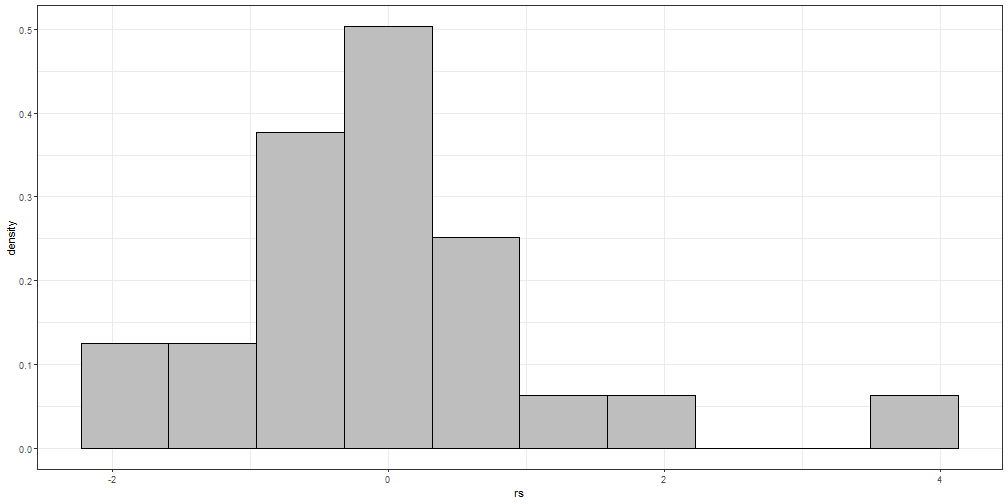
\includegraphics{cap08_files/figure-latex/unnamed-chunk-5-1.pdf}

\begin{Shaded}
\begin{Highlighting}[]
\NormalTok{dados }\SpecialCharTok{\%\textgreater{}\%} 
  \FunctionTok{group\_by}\NormalTok{(S,F) }\SpecialCharTok{\%\textgreater{}\%} 
  \FunctionTok{summarise}\NormalTok{(}\AttributeTok{Y =} \FunctionTok{mean}\NormalTok{(y)) }\SpecialCharTok{\%\textgreater{}\%} 
  \FunctionTok{ggplot}\NormalTok{(}\FunctionTok{aes}\NormalTok{(}\AttributeTok{x=}\NormalTok{F, }\AttributeTok{y=}\NormalTok{Y,}\AttributeTok{col=}\FunctionTok{as.factor}\NormalTok{(S)))}\SpecialCharTok{+}
  \FunctionTok{geom\_line}\NormalTok{()}\SpecialCharTok{+}
  \FunctionTok{labs}\NormalTok{(}\AttributeTok{x=}\StringTok{"Fungicida"}\NormalTok{,}\AttributeTok{y=}\StringTok{"Altura de plantas (cm)"}\NormalTok{,}\AttributeTok{col=}\StringTok{"Tratamento do solo"}\NormalTok{)}
\end{Highlighting}
\end{Shaded}

\begin{verbatim}
## `summarise()` has grouped output by 'S'. You can override using the `.groups`
## argument.
\end{verbatim}

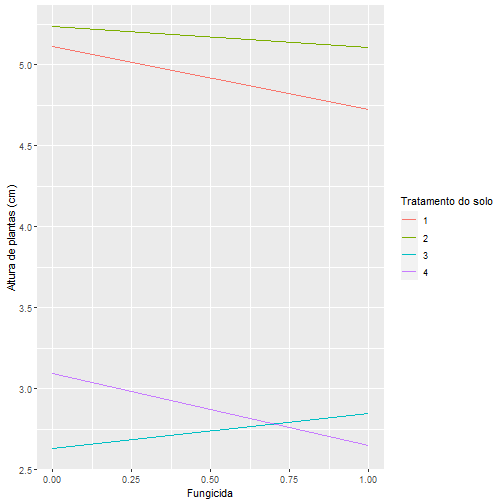
\includegraphics{cap08_files/figure-latex/unnamed-chunk-5-2.pdf}

\textbf{Utilizando ao pacrote ExpDes.pt, mais prático}

\begin{Shaded}
\begin{Highlighting}[]
\CommentTok{\# Carregando o pacote para análise de variância}
\FunctionTok{library}\NormalTok{(ExpDes.pt)}
\end{Highlighting}
\end{Shaded}

\begin{verbatim}
## 
## Attaching package: 'ExpDes.pt'
\end{verbatim}

\begin{verbatim}
## The following objects are masked from 'package:agricolae':
## 
##     lastC, order.group, tapply.stat
\end{verbatim}

\begin{Shaded}
\begin{Highlighting}[]
\CommentTok{\# Definindo o caminho do banco de dados}
\NormalTok{caminho}\OtherTok{\textless{}{-}}\StringTok{"https://raw.githubusercontent.com/arpanosso/ExpAgr\_2020/master/dados/solofungi.txt"}

\CommentTok{\# Entrada da dados}
\NormalTok{dados}\OtherTok{\textless{}{-}}\FunctionTok{read.table}\NormalTok{(caminho,}\AttributeTok{h=}\ConstantTok{TRUE}\NormalTok{)}

\CommentTok{\#Guardando os fatores (tratamentos de solo e fungicidas) e a variável resposta (y)}
\NormalTok{solos}\OtherTok{\textless{}{-}}\NormalTok{dados}\SpecialCharTok{$}\NormalTok{S}
\NormalTok{fungicida}\OtherTok{\textless{}{-}}\NormalTok{dados}\SpecialCharTok{$}\NormalTok{F}
\NormalTok{y}\OtherTok{\textless{}{-}}\NormalTok{dados}\SpecialCharTok{$}\NormalTok{y}

\CommentTok{\# Utilizando a função fat2.dic do pacote ExpDes.pt}
\FunctionTok{fat2.dic}\NormalTok{(solos,fungicida,y,}\AttributeTok{fac.names =} \FunctionTok{c}\NormalTok{(}\StringTok{"Trat\_Solo"}\NormalTok{, }\StringTok{"Fungicida"}\NormalTok{))}
\end{Highlighting}
\end{Shaded}

\begin{verbatim}
## ------------------------------------------------------------------------
## Legenda:
## FATOR 1:  Trat_Solo 
## FATOR 2:  Fungicida 
## ------------------------------------------------------------------------
## 
## 
## Quadro da analise de variancia
## ------------------------------------------------------------------------
##                     GL     SQ QM     Fc   Pr>Fc
## Trat_Solo            3 30.395  5 74.004 0.00000
## Fungicida            1  0.209  4  1.527 0.23439
## Trat_Solo*Fungicida  3  0.413  3  1.005 0.41607
## Residuo             16  2.191  2               
## Total               23 33.208  1               
## ------------------------------------------------------------------------
## CV = 9.42 %
## 
## ------------------------------------------------------------------------
## Teste de normalidade dos residuos (Shapiro-Wilk)
## valor-p:  0.6260575 
## De acordo com o teste de Shapiro-Wilk a 5% de significancia, os residuos podem ser considerados normais.
## ------------------------------------------------------------------------
## 
## Interacao nao significativa: analisando os efeitos simples
## ------------------------------------------------------------------------
## Trat_Solo
## Teste de Tukey
## ------------------------------------------------------------------------
## Grupos Tratamentos Medias
## a     2   5.173333 
## a     1   4.921667 
##  b    4   2.873333 
##  b    3   2.738333 
## ------------------------------------------------------------------------
## 
## Fungicida
## De acordo com o teste F, as medias desse fator sao estatisticamente iguais.
## ------------------------------------------------------------------------
##   Niveis   Medias
## 1      0 4.020000
## 2      1 3.833333
## ------------------------------------------------------------------------
\end{verbatim}

\end{document}
